
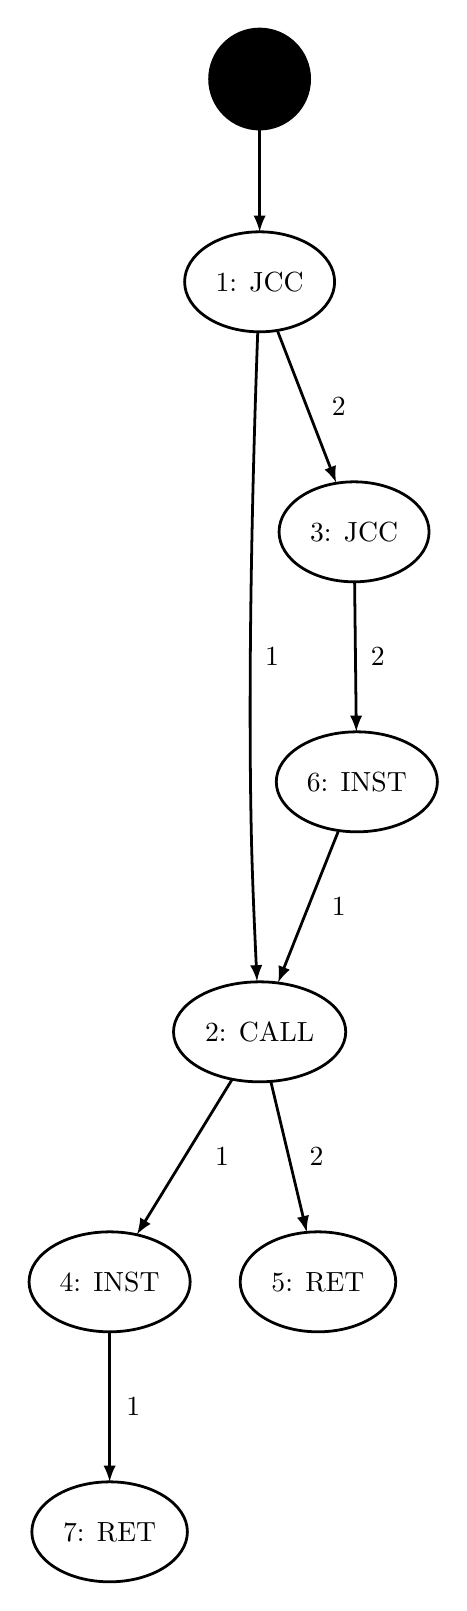
\begin{tikzpicture}[>=latex,line join=bevel,]
  \pgfsetlinewidth{1bp}
%%
\pgfsetcolor{black}
  % Edge: 2 -> 3
  \draw [->] (73.096bp,180.86bp) .. controls (65.027bp,167.71bp) and (53.498bp,148.92bp)  .. (38.842bp,125.04bp);
  \definecolor{strokecol}{rgb}{0.0,0.0,0.0};
  \pgfsetstrokecolor{strokecol}
  \draw (69.5bp,153bp) node {1};
  % Edge: 6 -> 7
  \draw [->] (117.2bp,359.61bp) .. controls (117.34bp,347.24bp) and (117.53bp,330.37bp)  .. (117.81bp,306.05bp);
  \draw (125.5bp,333bp) node {2};
  % Edge: 1 -> 6
  \draw [->] (89.395bp,450.45bp) .. controls (94.303bp,437.75bp) and (101.17bp,419.96bp)  .. (110.52bp,395.78bp);
  \draw (111.5bp,423bp) node {2};
  % Edge: 7 -> 2
  \draw [->] (111.42bp,270.45bp) .. controls (106.36bp,257.75bp) and (99.292bp,239.96bp)  .. (89.673bp,215.78bp);
  \draw (111.5bp,243bp) node {1};
  % Edge: 1 -> 2
  \draw [->] (82.321bp,449.87bp) .. controls (81.057bp,415.68bp) and (78.595bp,336.51bp)  .. (80bp,270bp) .. controls (80.303bp,255.64bp) and (80.951bp,239.66bp)  .. (82.069bp,216.21bp);
  \draw (87.5bp,333bp) node {1};
  % Edge: 0 -> 1
  \draw [->] (83bp,522.81bp) .. controls (83bp,514.79bp) and (83bp,505.05bp)  .. (83bp,486.03bp);
  % Edge: 2 -> 5
  \draw [->] (87.049bp,180.03bp) .. controls (90.041bp,167.49bp) and (94.175bp,150.17bp)  .. (99.963bp,125.92bp);
  \draw (103.5bp,153bp) node {2};
  % Edge: 3 -> 4
  \draw [->] (29bp,89.614bp) .. controls (29bp,77.24bp) and (29bp,60.369bp)  .. (29bp,36.05bp);
  \draw (37.5bp,63bp) node {1};
  % Node: 1
\begin{scope}
  \definecolor{strokecol}{rgb}{0.0,0.0,0.0};
  \pgfsetstrokecolor{strokecol}
  \draw (83bp,468bp) ellipse (27bp and 18bp);
  \draw (83bp,468bp) node {1: JCC};
\end{scope}
  % Node: 0
\begin{scope}
  \definecolor{strokecol}{rgb}{0.0,0.0,0.0};
  \pgfsetstrokecolor{strokecol}
  \definecolor{fillcol}{rgb}{0.0,0.0,0.0};
  \pgfsetfillcolor{fillcol}
  \filldraw [opacity=1] (83bp,541bp) ellipse (18bp and 18bp);
\end{scope}
  % Node: 3
\begin{scope}
  \definecolor{strokecol}{rgb}{0.0,0.0,0.0};
  \pgfsetstrokecolor{strokecol}
  \draw (29bp,108bp) ellipse (29bp and 18bp);
  \draw (29bp,108bp) node {4: INST};
\end{scope}
  % Node: 2
\begin{scope}
  \definecolor{strokecol}{rgb}{0.0,0.0,0.0};
  \pgfsetstrokecolor{strokecol}
  \draw (83bp,198bp) ellipse (31bp and 18bp);
  \draw (83bp,198bp) node {2: CALL};
\end{scope}
  % Node: 5
\begin{scope}
  \definecolor{strokecol}{rgb}{0.0,0.0,0.0};
  \pgfsetstrokecolor{strokecol}
  \draw (104bp,108bp) ellipse (28bp and 18bp);
  \draw (104bp,108bp) node {5: RET};
\end{scope}
  % Node: 4
\begin{scope}
  \definecolor{strokecol}{rgb}{0.0,0.0,0.0};
  \pgfsetstrokecolor{strokecol}
  \draw (29bp,18bp) ellipse (28bp and 18bp);
  \draw (29bp,18bp) node {7: RET};
\end{scope}
  % Node: 7
\begin{scope}
  \definecolor{strokecol}{rgb}{0.0,0.0,0.0};
  \pgfsetstrokecolor{strokecol}
  \draw (118bp,288bp) ellipse (29bp and 18bp);
  \draw (118bp,288bp) node {6: INST};
\end{scope}
  % Node: 6
\begin{scope}
  \definecolor{strokecol}{rgb}{0.0,0.0,0.0};
  \pgfsetstrokecolor{strokecol}
  \draw (117bp,378bp) ellipse (27bp and 18bp);
  \draw (117bp,378bp) node {3: JCC};
\end{scope}
%
\end{tikzpicture}

